\section{Eksempler}\label{sec:des-examples}
%\inline{Beskrivelse af eksemplet og hvordan det er relateret til problemet/modellen. Beskrivelse af løsning uden vores tid}


\subsection{Hajer og fisk på Wa-Tor} 
Vores første eksempel tager  udgangspunkt i et Lotka-Volterra predator-prey scenarie, som \citeauthor{wator}
har beskrevet i artiklen \citetitle{wator}\cite{wator}. Artiklen beskriver den
fiktive planet Wa-Tor, der har form som en torus og er fuldstændig
dækket af vand. Verdenen er inddelt i felter, som kan være tomme, indeholde en
fisk eller en haj\cite[20]{wator}. Følgende karakteristika beskriver fisk og hajers
opførsel.

\begin{itemize}
\item[\textbf{Fisk}]
Lever af plankton, en ressource som er uendelig. Hvis der er ét ledigt 
tilstødende felt, bevæger den sig til dette felt. Hvis der er flere ledige 
felter vælges et tilfældigt. Såfremt en fisk overlever 3 tidsskridt forplanter 
den sig.
\item[\textbf{Hajer}]
Såfremt der er fisk i et eller flere tilstødende felter, vil hajen bevæge sig 
til et af disse felter og spise fisken. Hvis der er ikke er nogen fisk i et af 
disse felter flytter hajen sig til et tilfældigt valgt ledigt felt. Hvis en haj 
ikke spiser i 3 tidsskridt dør den. Overlever den i 10 tidsskridt forplanter 
den sig.
\end{itemize}

For hvert tidsskridt vil alle fisk og hajer udføre en handling ud fra
ovenstående opførsel.
Til at initiere systemet skal der defineres en størrelse af verdenen,
samt hvor mange fisk og hajer der er til stede fra start. Disse fisk og
hajer placeres tilfældigt i verdenen.
Såfremt de initielle parametre for antal fisk og hajer understøtter en 
bæredygtig bestand forventer vi at se bestanden af henholdsvis fisk og hajer 
oscillerer afhængigt af hinanden.

Vi har valgt dette eksempel, da det er et klassisk simuleringsproblem der er enkelt og let forståeligt, men samtidig 
introducerer problemstillinger omkring synkronisering når det paralleliseres.  
Disse problemstillinger optræder fordi en opdatering af hvert felt er afhængigt 
af de omkringliggende felter, og vil derfor være afhængig af felter fra andre 
processer i grænsetilfælde. Ud over at være afhængig af information fra andre 
processer, kan en opdatering også påvirke data hos andre processer. Eksemplet er repræsentativt for de problemer der ligger i kategorien af continuous simulation, og viser at hvis vi kan bruge vores implementation af \des til simulering af dette eksempel vil man helt generelt kunne bruge det til continuous simulations.

\subsubsection{Før introduktion af et tidsbegreb i \pycsp}
For at simulere Wa-Tor verdenen i \pycsp hvori tidsbegrebet ikke er introduceret, er vi nødt 
til at udføre en synkronisering af de enkelte processers arbejde. Denne 
synkronisering kan ske ved brug af barrierer, hvor alle processer udfører en 
handling og mødes i barrieren før de fortsætter.

Vi har valgt at basere vores model på \citetitle{crew}\cite{crew}, hvor verdenen repræsenteres 
som en delt datastruktur og adgangen til denne styres med barrierer. I vores 
model er hver proces derved ansvarlig for en del af verdenen og tilgangen til 
den delte datastruktur sker ud fra CREW-princippet (Concurrent Read, Exclusive 
Write)\cite[5]{crew}, der styres vha. barrierer.  

I en mere ren \csp-model ville man foretage en direkte udveksling af data mellem 
processerne, og undgå den delte datastruktur vi har i vores model.  Vi har 
valgt denne model frem for den mere rene \csp model, da den klarlægger brugen af 
barrierer bedre.  Det bliver meget eksplicit i koden hvornår hvilke dele 
opdateres, og hvornår processerne venter i en barriere.

Vi deler verdenen lodret, hvor hver proces styrer en verdensdel. Hver proces 
gennemgår sin verdensdel og udfører en mulig handling for hver fisk og haj, dog 
vil fisk og hajer i de sidste to kolonner i hver verdensdel ikke bliver 
opdateret på nuværende tidspunkt. Dette skyldes at der kan opstå en race 
condition hvis disse to kolonner opdateres samtidig med de andre. Årsagen til 
dette er at både processen der er ansvarlig for kolonnerne, og processen 
umiddelbart til højre for den skal have mulighed for at flytte fisk og hajer fra og til dette område. 
Når denne 
opdatering er fuldført mødes processerne i en barriere, hvorefter hver proces 
opdaterer de to sidste kolonner. Herefter mødes processerne igen i barrieren, 
og når alle kolonner er opdateret kan der foretages en visualisering af de 
udførte opdateringer. Til slut mødes alle i en barriere igen før processerne 
kan begynde en ny iteration.

En repræsentation af opdelingen ses på \cref{fig:wator}. Her er verdenen 
opdelt mellem to processer, og de to kolonner mellem hver del opdateres i et 
separat tidsskridt.  

\begin{figure}
 \begin{center}
  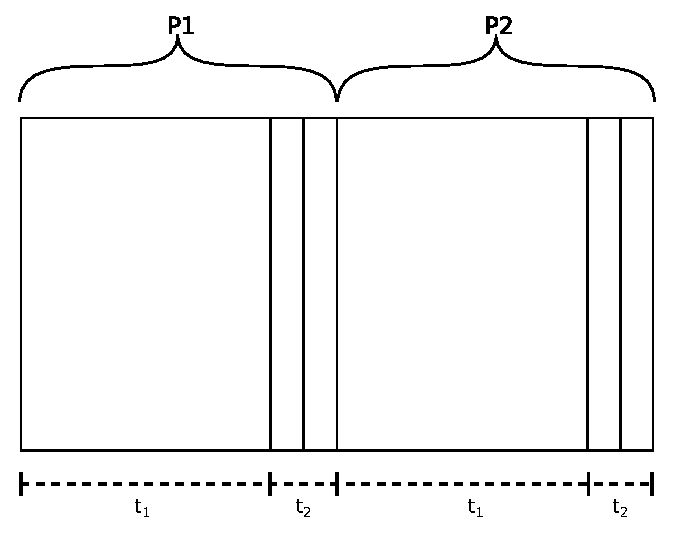
\includegraphics[scale=0.75]{images/wator}
  \caption{Opdeling af verdenen mellem to processer. Der er for hver verdensdel 
  to kolonner som opdateres i et separat tidsskridt.}
  \label{fig:wator}
  \end{center}
\end{figure}


\begin{figure}[hbtp]
\begin{minipage}{\linewidth}
\begin{lstlisting}[label=code:wator-worldpart,caption=Uddrag af processen 
  \code{worldpart} i Wator]
  @proces
  def worldpart (part_id, barR, barW):  
    ...  
    while True:
      #Calc your world part:
      main_iteration()
      barW(1)
      barR()
      #Update the two shadowcolumns
      for i in range(world_height):
        for j in range(2):
          element_iteration(Point(right_shadow_col+j,i))
      barW(1)
      barR()
      #visualize have single access
      barW(1)
      barR()
\end{lstlisting}

\begin{lstlisting}[label=code:wator-visualize,caption=Processen 
  \emph{visualize} i Wator]
@proces
 def visualize(barR,barW):
   for i in xrange(iterations):
     barW(1)
     barR()
     barW(1)
     barR()
     pygame.display.flip()
     barW(1)
     barR()
   poison(barW,barR)
\end{lstlisting}

\end{minipage}
\caption[test]{\code{barW(1)} og \code{barR()} er henholdsvis skrivning og læsning til og 
fra en barriere som defineret i \cref{sec:barrierer}.}
\end{figure}
Afviklingen af programmet sker ved at et antal worldpart-, en 
visualize- og en barrier-proces køres parallelt. Af 
\autoref{code:wator-worldpart} og \cref{code:wator-visualize}, ses det 
overordnede design af henholdsvis worldpart- og 
vizualize-processen.  
\subsubsection{Konklusion}
%\inline{konklusion hvordan var det at implementere og hvor stor parallelitet kan man opnå. }
Det var ikke svært at implementere et predator/prey simulering i \pycsp, men da store dele af koden bruges på at simulere  de forskellige fisk, og ikke på synkronisering, forventer vi ikke at introduktionen af tid i \pycsp vil medføre de store ændringer. 

Værd at bemærke er det store antal barrierekald i 
visualize-processen. Dette er til for at man kan benytte den samme barriere som 
worldpart-processerne. Alternativt kunne man have to barriere-processer; en til 
synkronisering af worldpart med vizualize, samt en som 
worldpart-processerne bruger til synkroniseringen af de to sidste kolonner. 

\subsection{Kunder i en bank}\label{bank-eksempel}
Et klassisk eksempel inden for \des er at simulere  en række kunder der alle 
ankommer til en butik, hvor de skal serviceres. Dette simple problem kan 
udvides til at modellere mange forskellige problemstillinger, der berører 
hvordan flowet ændrer sig hvis man varierer en eller flere parametre
i systemet. Programmeringssproget \simpy\footnote{\url{http://simpy.sourceforge.net/}}har, som et af deres 
eksempler, en simulering af kunder i en bank. \simpy bruger dette som et 
gennemgående eksempel, hvor de løbende udvider modellen, for at vise 
forskellige egenskaber ved \simpy. For at kunne sammenligne \simpy  med vores 
version, vil vi implementere to af eksemplerne med kunder 
i en bank i \pycsp.

I det simple tilfælde af eksemplet ankommer kunderne til banken på 
tilfældige tidspunkter.  De opholder sig i banken i et tilfældigt 
tidsrum, hvorefter de igen forlader banken. I dette eksempel kan der ikke 
uddrages meget information, men det viser hvordan en simpel model er opbygget i 
hhv.  \simpy og \pycsp for at håndtere tid.

I det andet eksempel er modellen udvidet med en servicedisk, hvilket giver at eksemplet bliver en M/M/1 kømodel\fxnote{Brian - er det relevant at snakke om kømodeller?}. Her skal alle 
kunderne betjenes af en servicemedarbejder, som kun kan ekspederes en kunde ad 
gangen. Alle kunder ankommer til banken på tilfældige tidspunkter  og stiller sig i 
kø for at blive serviceret. Det er igen et tilfældigt tidsrum som kunden bruger på at blive 
serviceret.  Dette er stadigt en meget simpel model, men med introduktionen af 
en begrænset ressource kan man uddrage information om den tilhørende kø, f.eks. 
kan der måles hvor lang det tager for hver kunde at blive betjent af 
servicemedarbejdere, samt hvordan køen opfører sig over tid. 

\subsubsection{Før introduktion af et tidsbegreb i \pycsp}

I \simpy opretter generatorfunktionen dynamisk en kundeprocess og  kører den parallelt med sig selv. Det vil  være nærliggende ligeledes at 
modellere eksemplet i \pycsp med kunder som en proces. I \pycsp er processerne mere statiske, gerne med en generator- og 
arbejderproces, hvor  arbejdet flyttes 
mellem processerne igennem kanaler. Vi har derfor ændret modellen så   
generatorprocessen i \pycsp er som i \simpy, men vi introducerer en bankproces i stedet for en kundeproces, og lader kunderne være arbejdet der flyttes mellem dem. 
I \pycsp findes muligheden for at oprette processer dynamisk med funktionen \code{spawn}, og man kunne derfor god lade generatoprocessen oprette kundeprocesser dynamisk, men vi ønsker ikke kun at kopiere eksemplet fra \simpy til \pycsp, men også konvertere eksemplet så der overholder stilen for et program skrevet til \csp. 

Mens \simpy kalder kundeprocessen fra generatoren og lader denne stå for håndteringen af kunden 
og den tid hun befinder sig i banken, kender bankprocessen i \pycsp ikke tid som 
sådan. Bankprocessen skal derfor selv vedligeholde en liste med kunderne, der findes inden i banken og til hver 
tidskridt vide hvilke kunder der skal forlade den. 

Tiden er igen modelleret ved brug af barrierer. I 
stedet for at have de to kald til barrieren som den kræver, lige efter hinanden, lader 
vi bankprocessen gå ind i barrieren i starten af tidsskridtet, og så modtage 
kunder, indtil bankeprocessen modtager det andet kald fra barrieren (se\cref{bank-alternation-imp}). Dette er nødvendigt for at lade banken have 
mulighed for at modtage et vilkårligt antal kunder i samme tidsskridt, samt 
vide hvornår der ikke vil komme flere kunder.  Vi kan ræsonnere os frem til at 
barrieren stadig virker efter hensigten ved  simpel indsigt.
For at generatorprocessen kan komme foran med et tidsskridt og sende en kunde i et forkert tidsskridt,
skal den have fuldført begge begge kald til barrieren, mens bankprocessen ikke 
har modtaget et kald fra barrieren. Barrieren vil dog ikke modtage kald fra 
nogle, før den har  kaldt bankprocessen. Derfor må generatorprocessen vente i 
sit første kald til barrieren, indtil banken har modtaget sit kald fra 
barrieren, før den kan sende en ny kunde.
Når bankprocessen har modtaget et kald fra barrieren er den ikke længere villig 
til at modtage kunder, før i det efterfølgende tidsskridt. Vi kan bruge samme 
ræsonnement for at bankprocessen heller ikke kan komme et 
tidsskridt foran generatorfunktionen, og derfor virker barrieren stadigt som 
forventet. 

\begin{lstlisting}[float=hbtp,label=bank-alternation-imp,caption=Modtage en 
  kunde eller barrierekald i Bankprocessen]
while True:
		(g,msg) = Alternation([{
		barrierREADER:None,
    customerREADER:None
    }]).select()
		if g == barrierREADER:
			break
    elif g == customerREADER:
			heappush(customers,(time+msg.waittime,msg))
\end{lstlisting}


I det mere avancerede eksempel hvor kunderne skal tilgå den samme begrænsede 
ressource dannes en kø. Denne kan i \pycsp modeleres på flere måder, afhængigt 
at hvilken proces der skal have ansvaret for at vedligeholde køen. En metode er 
internt i en proces at have en liste af kunder der venter, og lade det være 
processens ansvar at håndtere denne liste som en kø. Processen med ansvaret for køen kan 
så enten være den begrænsede ressource, eller en separat proces hvis eneste 
formål er at vedligeholde køen. For nyligt\footnote{d. 22. december 2009} er 
der i \pycsp blevet introduceret bufferkanaler\cite{pycsp-r147}, og 
disse kan også bruges som en kø. Dermed kan man modellere sin proces uden 
hensyntagen til håndtering af køen, og blot lade processen læse fra kanalen når den er klar. Vi har i dette eksempel valgt 
at lade køen være repræsenteret ved en bufferkanal, da denne  kræver 
færrest linjer kode, men den kunne lige så godt være repræsenteret som en liste 
i servicedisk processen.


\subsubsection{Konklusion}
Ved at se på implementeringen af de to eksempler af kunder i en bank sammenholdt med implementeringen i \simpy, kan man se at \des  egner sig godt til 
simulering disse problemer, og fra eksemplet kan man se at der findes meget kode til 
vedligeholdelse af de interne tidsvariabler, som \simpy ikke har behov for. Det drejer sig 
om kode der sørger for at hver proces kender tiden, samt at den er 
synkroniseret på tværs af processerne. Vi forventer derfor at koden skal kunne 
simplificeres i \pycsp med tid, så det bliver lige så simpelt at implementere som i 
\simpy. 

I \simpy findes begrebet ressource direkte i sproget, som en type og servicedisken er blot et objekt af denne type. 
En ressource i \simpy bruges til modellering af en begrænset ressource. Ved oprettelsen af ressourcen angives hvor mange der samtidigt kan tilgå den begrænsede ressource, og ressourcen står selv for at adgang til ressourcen samt den tilhørende kø, der eventuelt måtte opstå. 
I \pycsp modelleres servicedisken som en separat proces, og 
bankprocessen er derfor reduceret til blot at sende kunden videre til 
servicedisken og lade kanalen håndtere køen. 

En ulempe ved brugen af bufferkanaler som en kø er, at kanalen har en fast størrelse på sin buffer, som 
angives når kanalen oprettes. Man kan dermed risikere en deadlock ved brug af bufferkanaler sammen med barrierer. Dette opstår hvis ikke processen i samme 
tidsskridt kan foretage transmissionen og kalde barrieren.
Det kan løses med en \code{alternation} og \code{skip guard}, men så 
skal bankprocessen håndtere fejlede forsendelser og må nødvendigvis introducere en 
sekundær kø hvilket gør brugen af en bufferkanal overflødig. For undgå dette har vi i vores tilfælde valgt blot at 
angive en maksimal størrelse på bufferen som er større end det totale antal 
kunder banken modtager. \fxnote*{RS: Afhænger af den forrige fixme om M/M/1}{Dette medfører at det ikke længere er en teoretisk korrekt M/M/1 kømodel, da denne specifikt angiver at køen skal have mulighed for at have uendelig længde. I praksis er det ikke et problem da vi blot kan ræsonnere os frem til at køen ikke bliver fuld.}

